\chapter{Application design and implementation}
\label{chap:design}

\par For a clear application structure with different layers each providing specific services, I utilize Object Oriented Programming. It is a paradigm based on objects, meaning sets of data and procedures neatly packed together. The four principles on which it is built on are encapsulation, inheritance, polymorphism and abstraction \cite{Blaschek1994}.
\par Encapsulation means that the data is bundled together in one coherent package. In the case of classes it means that the data and the methods provided to manipulate them are under one roof, with possible limitations providing a way to minimize outside access.  
\par Inheritance provides the ability for one instance to derive the attributes and functionalities of other classes, enabling generalization. 
\par Polymorphism builds upon the concept of generalization, making it possible to access multiple types of objects through one common interface. This can usually occur in two different scenarios. The first one, static, is at compile time, for example method overloading, which is using the same function name with multiple signatures. The second, dynamic, is achieved at runtime, using a common derived interface, the exact type of an object will only be known when created. 
\par Abstraction is the concept of hiding unnecessary complexities, by moving  implementation details under an umbrella object. This can happen in multiple ways, depending on what scenario is it used in, like data oriented or object implementation. 
\par With the help of OOP I use layered architecture, similar to the Model View Controller design pattern, achieving a clear structure, with clear segmentation of responsibilities as seen in image \ref{fig:umldiagram}.

\begin{figure}
    \centering
    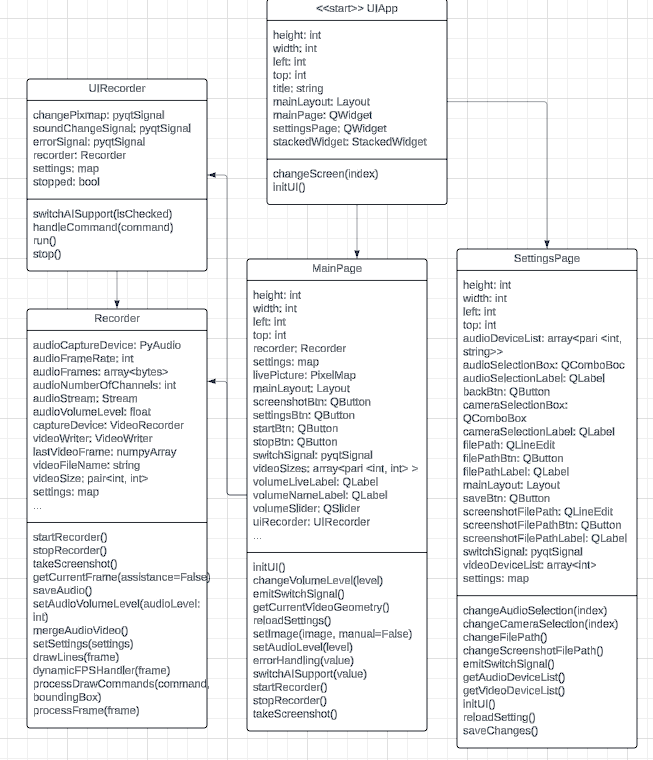
\includegraphics[width=0.5\linewidth]{figures/UML-Diagram.png}
    \caption{UML class diagram showing the relationships between the layers, made with \cite{lucidchart}}
    \label{fig:umldiagram}
\end{figure}

\par The layering enables the application to have three distinct parts, with different responsibilities. The top layer is the view unit, which is responsible for setting up the graphical user interface, with which the user interacts. Under it comes the controller layer, which includes the logic behind the application features. At the bottom the data layer is present, which retrieves the images and the audio.
\par While the top two layers are clearly present in the application, seen in image \ref{fig:umldiagram}, the last one implemented with the help of the opencv pyaudio and wave modules, in order to retrieve and save the data. Objects from these modules are saved in the Recorder class, the controller, and they act as repositories, a middleman for interacting with data.
\par To create a clear object for the logical steps, I utilize the facade design pattern \cite{facade} in the Recorder, hiding most of the complexities behind three simple functions: start, stop and getCurrentFrame. With the help of some parameters and setter functions, the controller can simply be used by the upper layer.

\section{Graphical User Interface}
\label{sec:designsec1}

\par The Graphical User Interface utilizes the signal based communication of the QT framework, for inter-widget discussion. This is an event based system, which allows independent objects to communicate with each other \cite{qtSignal}. With the help of this functionality, since it allows child to parent communication, the pages are broken down to independent objects, with a master class holding them together, providing an architecture where adding more pages is quite simple. To overcome the complexities which come with such a solution, two design patterns are used, namely the Composite and the Mediator, both of which are represented in the UI design in image \ref{fig:uidesignpattern}.

\begin{figure}
    \centering
    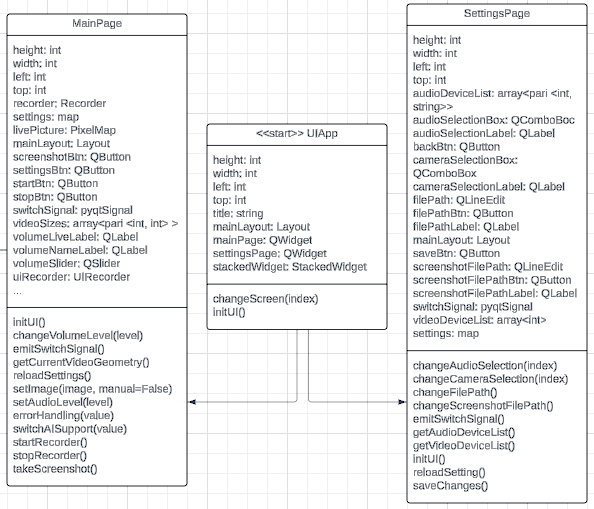
\includegraphics[width=0.6\linewidth]{figures/UIDesignPattern.png}
    \caption{Main design of the Graphical User Interface, made with \cite{lucidchart}}
    \label{fig:uidesignpattern}
\end{figure}

\par The composite design pattern states that the structure of what you are building can be represented in a tree, like a box containing more boxes and so on \cite{composite}. This is clearly present in the UI design \ref{fig:uidesignpattern}, where the main element is built from different page blocks, showing one at a time. 
\par The Mediator design pattern is used to keep the dependencies of different objects in check by not letting them directly talk to each other, only through third object, the mediator\cite{mediator}. This role is also up to he UIApp element, since the objects from which its built do not know about each other, they have to invoke the other through the the third party when switching pages.  

\begin{figure}
    \centering
    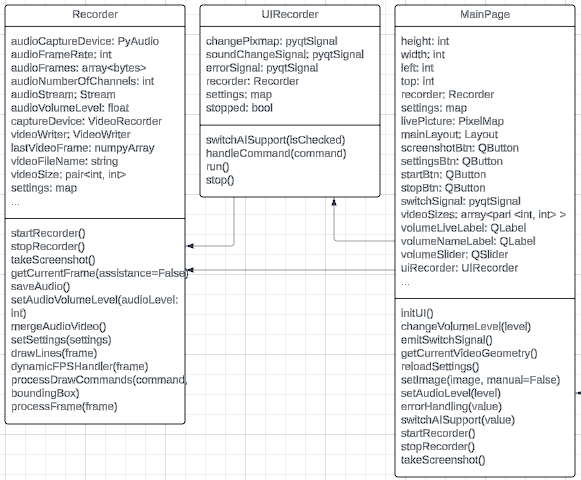
\includegraphics[width=0.6\linewidth]{figures/UIRecorder.png}
    \caption{The design of calling the controller layer in UI, made with \cite{lucidchart}}
    \label{fig:UIRecorder}
\end{figure}

\par Since the QT framework by default runs on one thread, when updating the live feed, the rest of the application becomes near unusable, since the recorder is always running. To combat this the Main page will not call the Recorder directly, instead creating a QThread object, UIRecorder, as can be seen in image \ref{fig:UIRecorder}.
\par This complicates the communication between the two view and controller layers, so in order to solve the problems the Observer design pattern \cite{observer} is utilized with the help of the already mentioned QT signaling system. This is achieved by the Main page subscribing to the changePixmap slot of the UIRecorder, which will send the retrieved frame back in an event based fashion.
\par The GUI has a minimalist look, providing the interactive elements in rows, using the Grid system of QT. In the Main page, the first row contains the live feed, the second the volume slider, the third an empty label, used for pop-up messages and the final row the navigation and functionality buttons as seen in the first image in figure \ref{fig:PageLooks}.
\par The Setting page is built with the same design in mind. The different sections occupy two rows each and are horizontally centered, while the last row contains the two buttons, one for saving the changes and one for navigating back to the Main page as seen in the second image \ref{fig:PageLooks}.

\begin{figure}
    \centering
    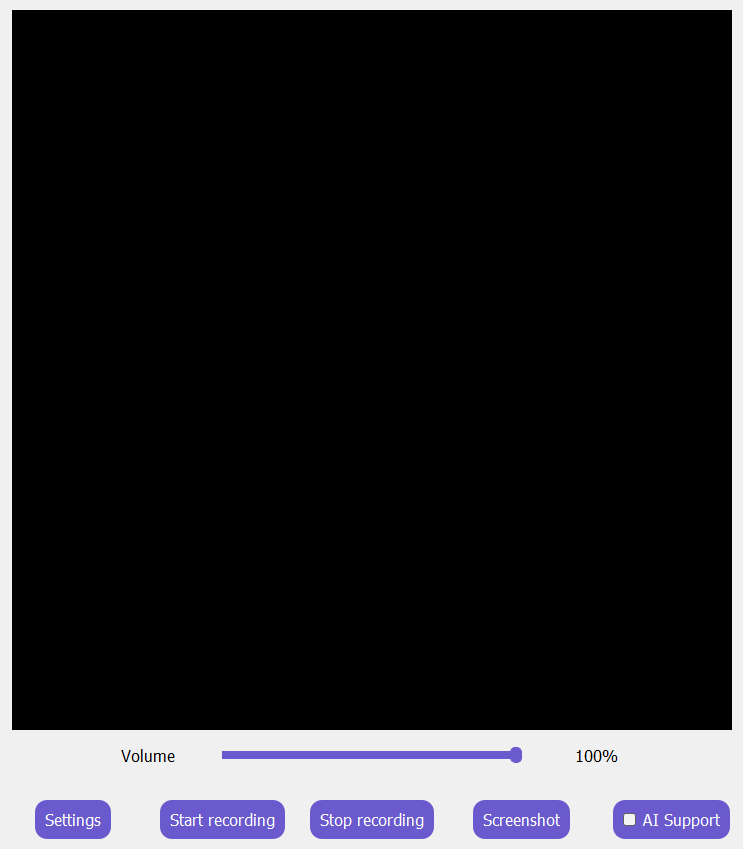
\includegraphics[width=0.35\linewidth]{figures/MainPage.png}
    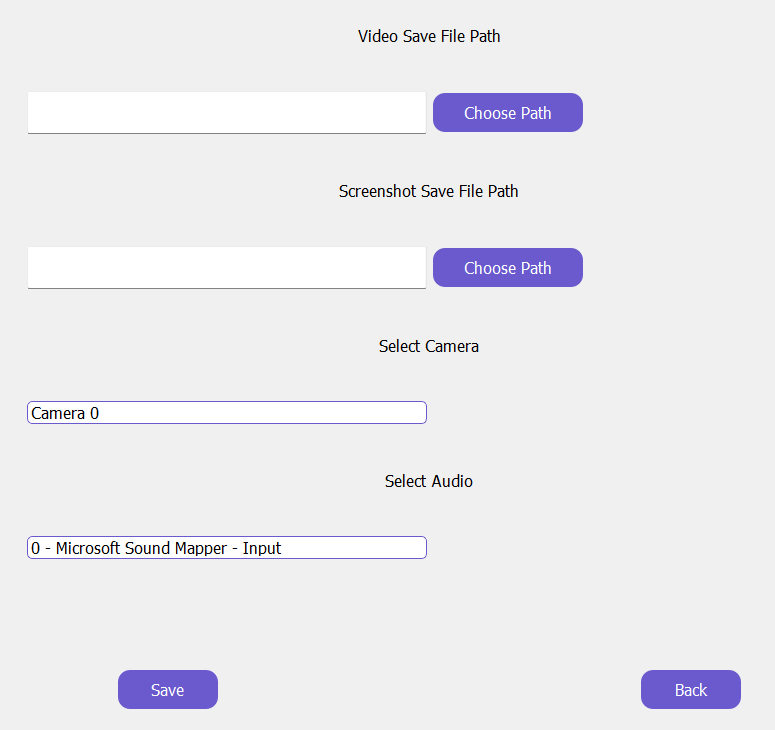
\includegraphics[width=0.45\linewidth]{figures/SettingsPage.png}
    \caption{The layout of the main page}
    \label{fig:PageLooks}
\end{figure}

\section{Image processing implementation}
\label{sec:designsec2}

\begin{figure}
    \centering
    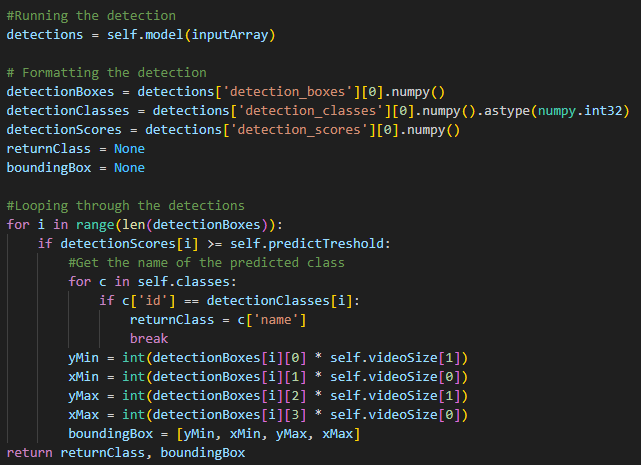
\includegraphics[width=0.5\linewidth]{figures/PredictionImplementation.png}
    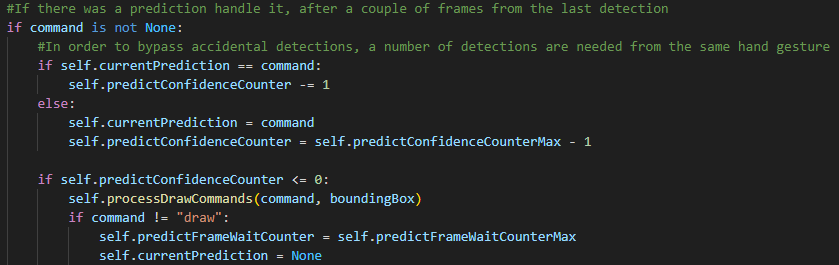
\includegraphics[width=0.5\linewidth]{figures/ConfidanceCount.png}
    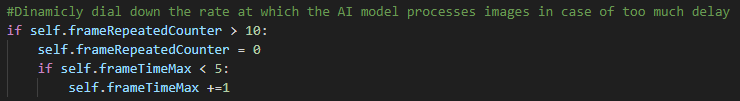
\includegraphics[width=0.4\linewidth]{figures/PredictionDialDown.png}
    \caption{Code snippets from the hand gesture prediction part}
    \label{fig:AIImplementations}
\end{figure}

\par The image processing is contained within the Recorder object. As mentioned before a deep learning model is used to detect the position and category of five hand gestures. This model is loaded from the start in order to be readily available when needed. The detection is done in the getCurrentFrame method, with a parameter toggling the use of it. It is done in two waves, the first being predicting the classes and bounding boxes. This is simply done by running the AI model, then retrieving the necessary information, than multiplying the relative bounding boxes from the model with the image dimensions as can be seen in  the first image from figure \ref{fig:AIImplementations}.
\par In order to minimize ghost detections and provide some breathing room between hand gestures, two counters are implemented, one calculating similar detections in a row and one for waiting after a successful hand gesture was detected, seen in image two \ref{fig:AIImplementations}.
\par For maximizing the fps in the video a dynamic dial is implemented in image three \ref{fig:AIImplementations}, which will increment a counter, stating how many frames have to skipped between model uses up to a maximum of five in order for the AI assistance to be usable. 

\section{Fixing fps count dynamically}
\label{sec:designsec3}

\par Since the recording of the audio and visual data is done separately, keeping a steady fps is needed for merging them correctly at the end. For this reason I implemented a simple fps handler as seen in image \ref{fig:FpsHandler}. With two time variables at the beginning and end of the frame calculations, it calculates how many milliseconds have passed, than compares that with the value of the camera's FPS. If the current running time is too slow, the current frame is repeated and a new audio batch is saved to keep up.

\begin{figure}
    \centering
    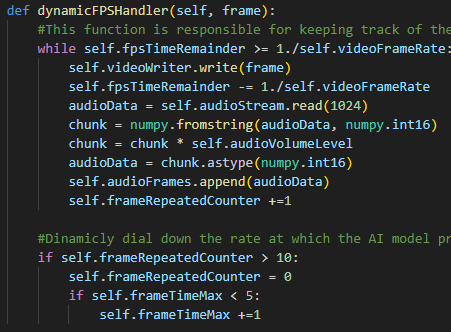
\includegraphics[width=0.4\linewidth]{figures/FpsHandler.png}
    \caption{Repeating frames to keep up with the cameras fps}
    \label{fig:FpsHandler}
\end{figure}

\section{Error Handling}
\label{sec:designsec4}

\par The error handling inside the application is done using try/except statements in the controller. In case of an exception a value will be returned to the UIRecorder, which will reset the controller if the issue occurred during recording, stop itself and send the value to the main page, where message will be presented to the user, depending on the integer. The messages are shown with the help of the QTimer object, which enables the application to clear the message label after a certain period of time. An example of an exception catching and the decoding of the integer value to a user message can be seen in images \ref{fig:ErrorHandling}.

\begin{figure}
    \centering
    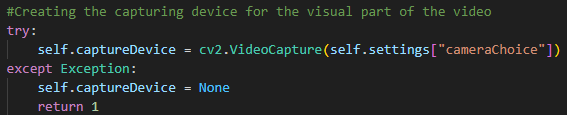
\includegraphics[width=0.4\linewidth]{figures/TryExcept.png}
    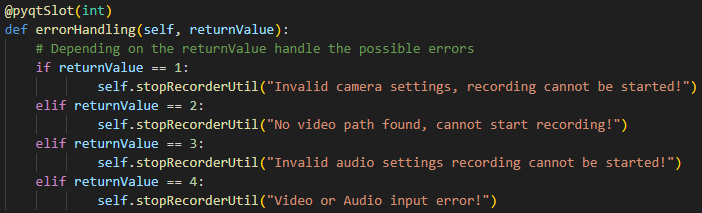
\includegraphics[width=0.4\linewidth]{figures/ErrorDecoding.png}
    \caption{Error handling in the controller and view layers}
    \label{fig:ErrorHandling}
\end{figure}

\section{Functionality implementation}
\label{sec:designsec5}

\subsection{Recording implementation}
\label{sec:designsec5subsec1}

\par The video recording starts with the initialization of the thread UIRecorder from the main page, which will initialize the opencv and pyaudio object in the controller layer and call the getCurrentFrame method of the Recorder class in while loop, until its stopped. From here the image is transformed to QImage, the image class of the QT framework, to be sent back to the main page and presented to the use, as shown in the first image in figure \ref{fig:RecordingCode}.
\par In the controller layer, the retrieval of the data done simply by reading values from the pyaudio and VideoCapture "repository" objects, after which comes the image processing part if it enabled. The next step of the getCurrentFrame function is saving the processed image directly to a file, and the audio to a numpy array, after it has been multiplied by the audio level variable, a number between 0 and 1.
\par At the end of the function we call the fps handler portion before returning the current frame and the retrieved hand gesture class as command to the UIRecorder, for it to forward the changes to the UI for user feedback as shown in the second image \ref{fig:RecordingCode}.
\par When the recording is stopped, the command cascades down from the view to the controller layer, where every variable will reset and as a final step the audio file saved and merged with the visual. The merging is done with the help of the moviepy module, which loads both temporary files, concatanetes the audio to the visual and outputs a final mp4 file, image three \ref{fig:RecordingCode}.

\begin{figure}
    \centering
    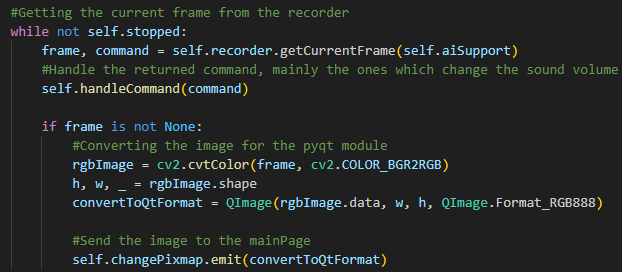
\includegraphics[width=0.4\linewidth]{figures/UIRecorderWhile.png}
    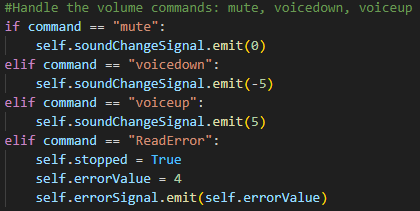
\includegraphics[width=0.4\linewidth]{figures/CommandHandling.png}
    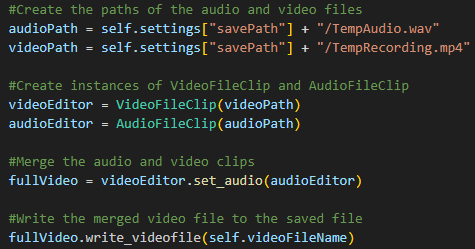
\includegraphics[width=0.4\linewidth]{figures/Merging.png}
    \caption{Recording implementation}
    \label{fig:RecordingCode}
\end{figure}

\subsection{Screenshot implementation}
\label{sec:designsec5subsec2}

\par For better performance in this functionality the current frame is always saved in the Recorder object, so only an image write has to be done with the help of the opencv module's imwrite method. 

\subsection{Volume change implementation}
\label{sec:designsec5subsec3}

\par The level change in the audio data is done by multiplying it with a values between 0 and 1 as mentioned in \ref{sec:designsec5subsec1}. The change of the audio level can be separated into two different scenarios. The first one is done with the slider found in the main page. In this case a function is connected to the slider in an event based fashion, which will directly set the volume variable of the Recorder object.
\par The second case is via the hand gesture controls. After the successful prediction of the class, that class is sent back to the UIRecorder as command, which will decode it, and send back integer values to the main page, as seen in image two \ref{fig:RecordingCode}. That value is sent as the parameter to the same function from the first case, from where the steps become the same as before. The up and down propagation of the data was an intentional design choice, in order to avoid writing almost duplicate functions for the variable change in the MainPage , which would have been necessary otherwise, since the UI elements are event based, so changing the slider values would call the first case no matter what.
\par Every time a change occurs the current volume level is stored, the only exception being in the case of mute, when the variable is simply put to zero or to the stored value, depending on the initial audio level.

\subsection{Changing the settings}
\label{sec:designsec5subsec4}

\begin{figure}
    \centering
    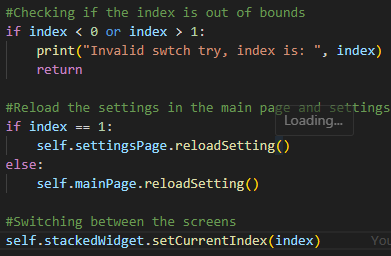
\includegraphics[width=0.4\linewidth]{figures/ScreenChange.png}
    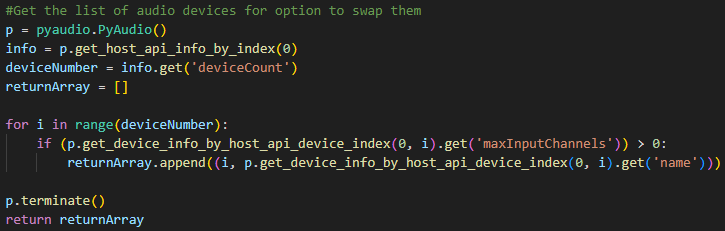
\includegraphics[width=0.4\linewidth]{figures/MicrophoneList.png}
    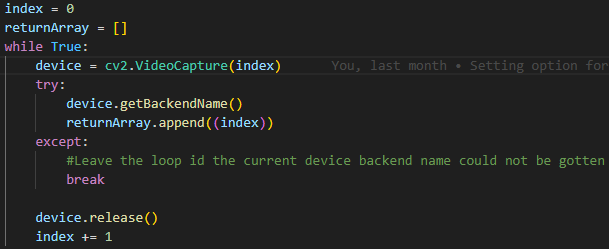
\includegraphics[width=0.4\linewidth]{figures/CameraList.png}
    \caption{UIApp screen change and settings implementations}
    \label{fig:ScreenChange}
\end{figure}

\par Switching from one page to the next is done with the help of QT signal as discussed in \ref{sec:designsec1}, by sending an integer value, the index of the current page, to the UIApp mediator. This class will than refresh the settings, by loading them from the json file, and change the stacked widget index, changing the page which is shown to the user, as shown in the first image \ref{fig:ScreenChange}. 
\par For choosing the path for the video and screenshot folder I use the tKinter module, which opens the File explorer in windows. From there the folder is chosen, and path is written in the text field. For the microphone options I retrieve the available devices from the pyaudio module. For the camera options, since there is no built in functionality, I try to open a VideoRecorder with different indexes until one that fails, creating a list if eligible indexes for working cameras. The implementations are presented in images two and three \ref{fig:ScreenChange}.
\par When the settings have been chosen the user can press the Save button which will save them in a json file.

\subsection{Drawing implementation}
\label{sec:designsec5subsec5}

\begin{figure}
    \centering
    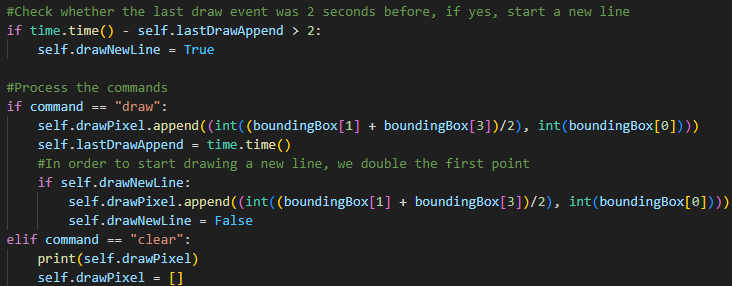
\includegraphics[width=0.4\linewidth]{figures/PointSaves.png}
    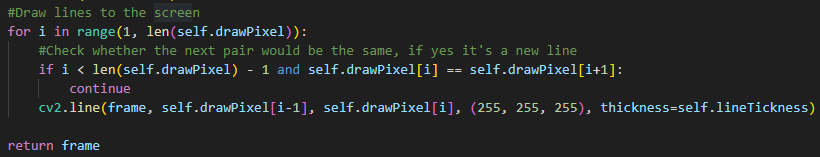
\includegraphics[width=0.4\linewidth]{figures/LineDrawings.png}
    \caption{The implementation details of the drawing functionality}
    \label{fig:DrawingImplementation}
\end{figure}

\par The drawing functionality is driven by the fourth and fifth hand gestures shown in figure \ref{customDataset}, and it is a special case in the prediction process, since this gesture will not create a pause between detection for the sake of a smoother drawing.
\par For every predicted draw class, the top middle point is calculated from the bounding box coordinates and then saved in an array. This means that for clearing the screen a simple clear of the point array is enough. To show the drawing the application iterates through these points and draw lines between them with the help of the opencv module, shown in the first image \ref{fig:DrawingImplementation}. This results in a continuous figure even when predictions are slow due to hardware limitations. In order to be able to start multiple figures, if there was a delay between draw class predictions, the middle point is saved twice, than at the draw stage checked, creating one skip. This achieves a break in the line, so the whole drawing will not be continuous, as seen in image two \ref{fig:DrawingImplementation}.
\par Whenever we have points saved the lines have to be drawn, so the corresponding function is called at every step, and since the method just returns when the array is empty, it is called whether or not the AI assistance is turned on, for the sake of a cleaner code.